\section{\Sys 编译器}
\label{sec:compiler}
本节介绍 \sys 编译器。它以计算图及其对应的推理配置为输入，生成同时针对目标配置与底层 GPU 架构优化的 \graph。整体编译流程如 \Cref{fig:compiler_workflow} 所示。

\begin{figure*}
    \centering
    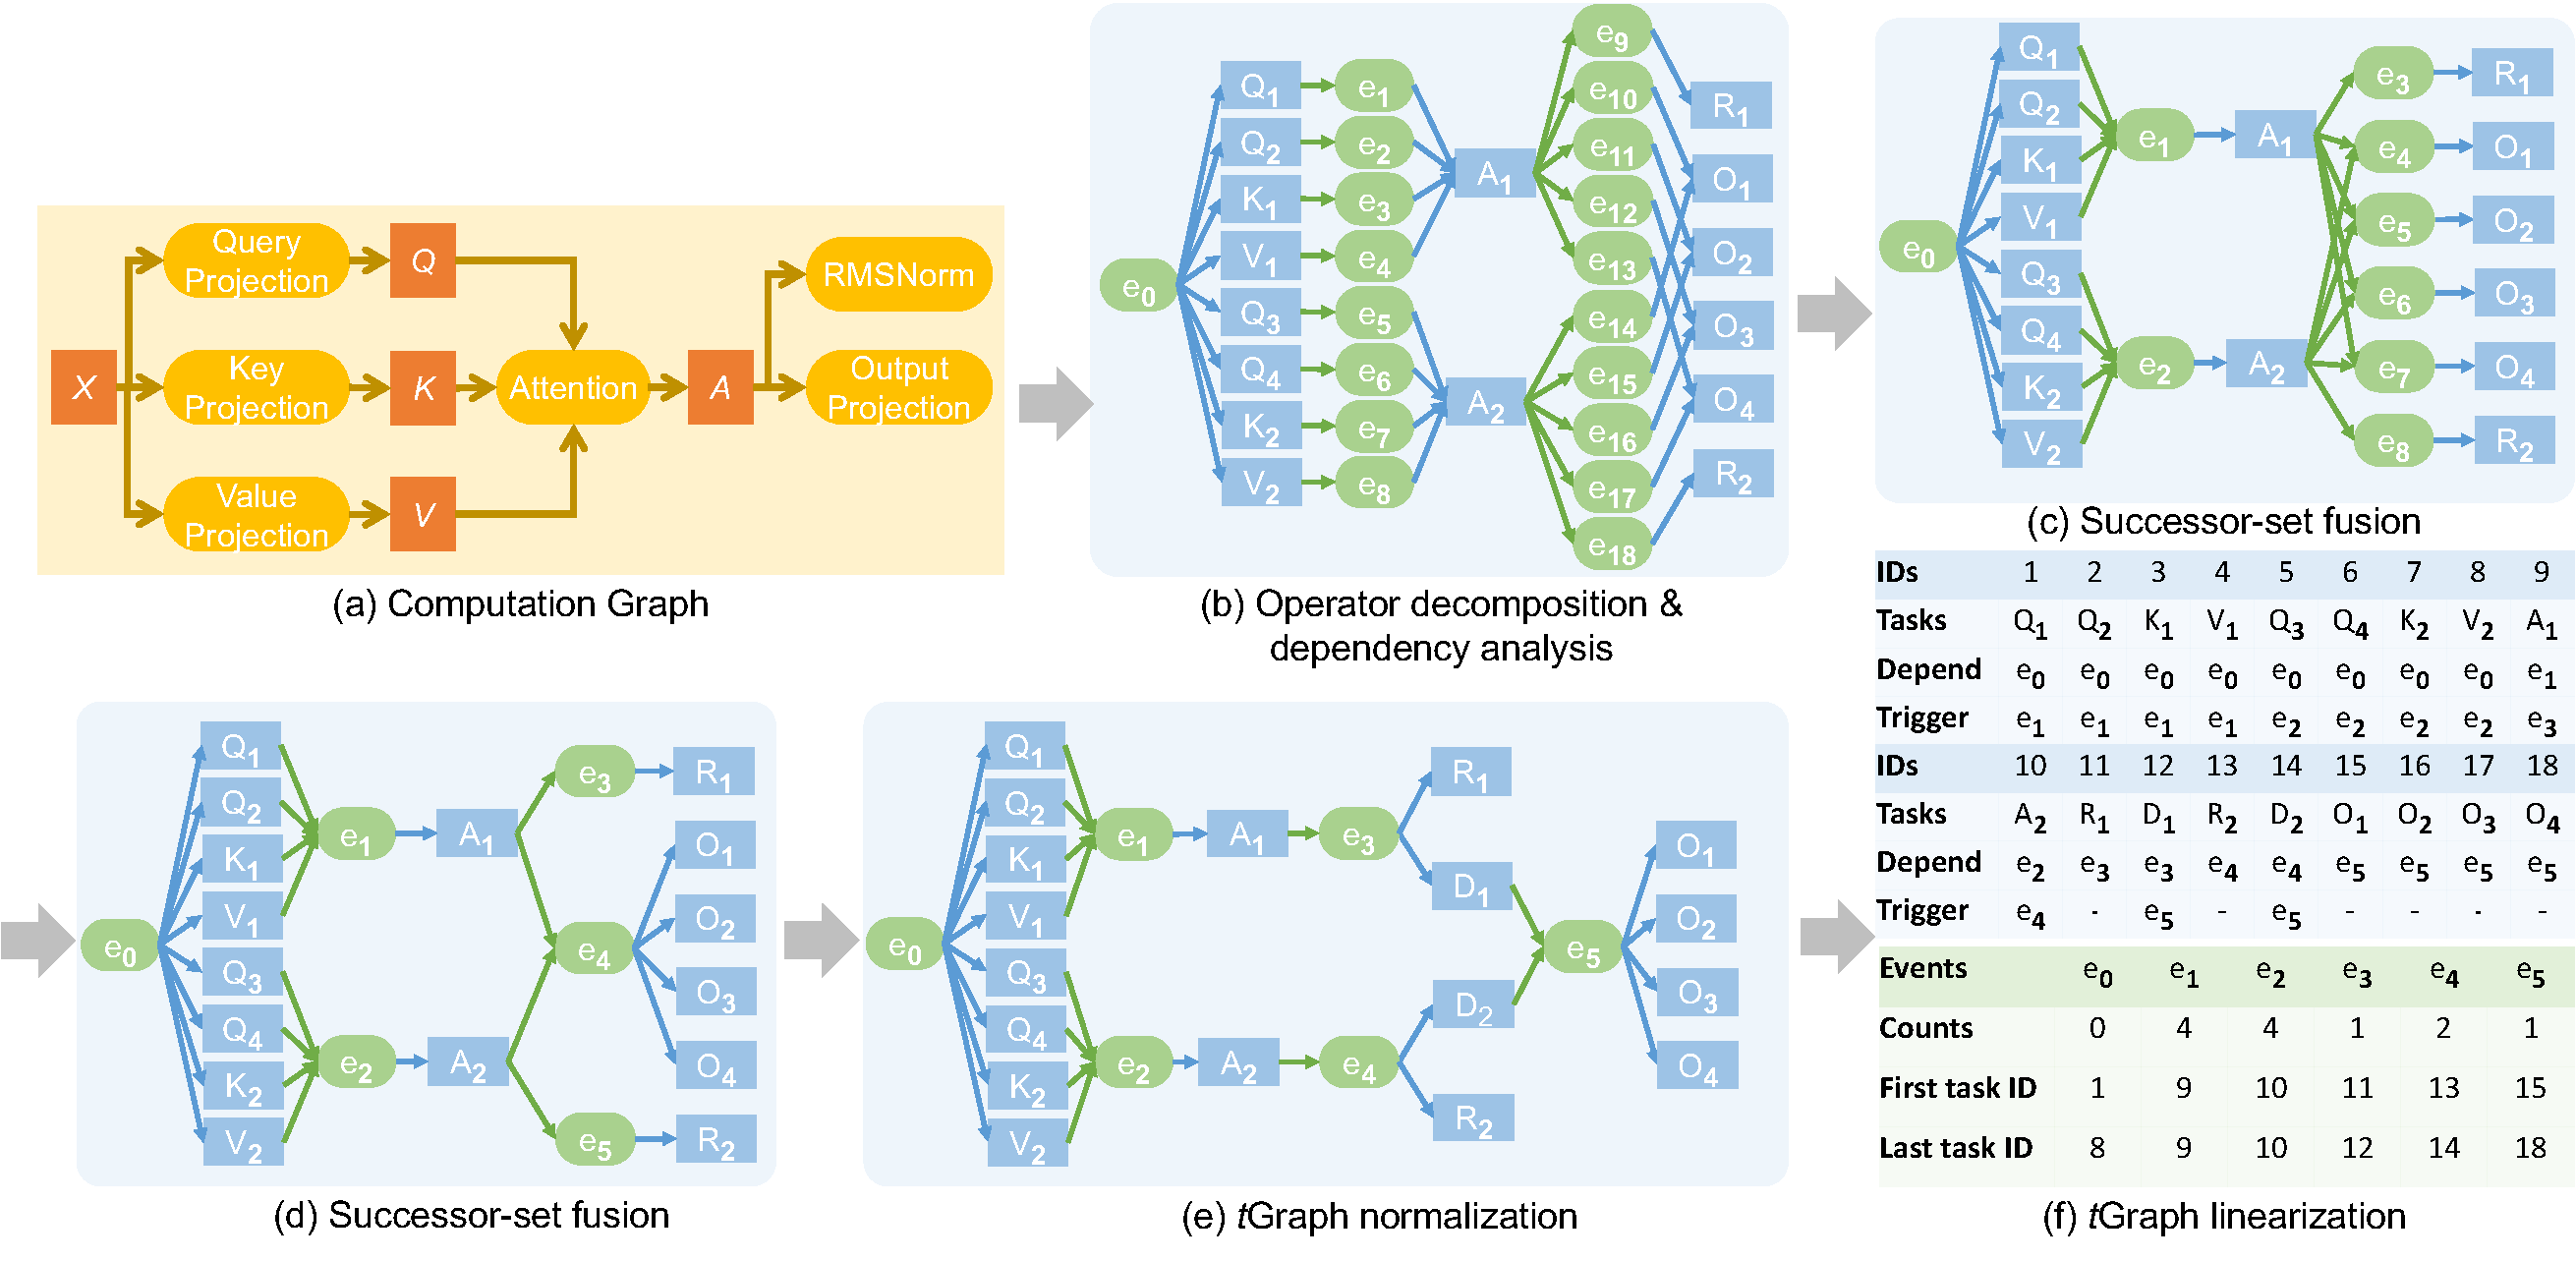
\includegraphics[scale=0.39]{figs/compiler_workflow_v3.pdf}
    \vspace{\captionvspace}
    \caption{\sys 编译器工作流。(b) 中的 $Q$、$K$、$V$、$A$、$O$ 和 $R$ 分别表示 query projection、key projection、value projection、attention、output projection 与 RMSNorm 被分解后得到的任务集合。(e) 中的 $D_1$ 与 $D_2$ 是在 \graph 规范化阶段插入的哑任务，用于保证每个任务都只有一个触发事件。最后，(f) 展示了 \Sys 如何对 \graph 进行线性化，并将任务与事件以统一的规范格式存储在 GPU 内存中。}
    \vspace{\captionvspace}
    \label{fig:compiler_workflow}
\end{figure*}

\subsection{\graph 生成}
\paragraph{算子分解。}
\sys 编译器通过对算子输出张量进行 {\em 切分}，把输入计算图中的每个算子分解成一组任务，使不同任务负责输出中彼此 {\em 不重叠} 的区域，并可以在多个 SM 上并行执行。多数张量代数算子都可以沿多个输出维度切分。例如，一个矩阵乘法的输出既可以沿行方向切块，也可以沿列方向切块，以暴露更多并行性。

切分策略的性能同时依赖问题形状与目标 GPU 架构。为了找到高效方案，\sys 优先选择那些能最小化从 device memory 向 shared memory 读入数据量的切分方式，因为访问 device memory 的代价显著高于访问 shared memory，且也高于在 CUDA core 或 tensor core 上执行计算。默认情况下，\sys 生成的任务数量会与 SM 数量成比例，以促进执行阶段的负载均衡。系统也向用户暴露接口，允许按输出维度指定并行度，从而自定义切分策略。

\paragraph{依赖分析。}
\Sys 使用 {\em event} 来表示任务之间的依赖。对于共享同一张量的两个算子，\sys 会枚举它们之间所有任务对，并仅在任务 $t_1$ 产出的输出区域与任务 $t_2$ 消费的输入区域发生重叠时，为该任务对 $(t_1, t_2)$ 引入一个事件 $e$。这一事件表示：只有当 $t_1$ 完成并产出所需数据后，$t_2$ 才能开始。为此，\sys 会在 \graph 中插入两条边 $(t_1, e)$ 与 $(e, t_2)$。这种细粒度依赖分析既完整保留了 producer-consumer 关系，又尽可能暴露出彼此独立任务之间的并行性。

\paragraph{事件融合。}
\Sys 进一步使用两类互补的事件融合来消除冗余同步点，并简化构造出的 \graph：{\em 后继集合融合} 与 {\em 前驱集合融合}。对于任一事件 $e$，记 $\er{InTasks}(e)$ 为触发该事件的任务集合，$\er{OutTasks}(e)$ 为依赖该事件的任务集合。借助这两个集合，我们可以判断不同事件是否具有相同依赖结构，从而合并。

第一类是 {\em 后继集合融合}。如果多个事件面向同一组后继任务，那么这些任务只有在所有相关事件都激活后才能执行，把它们分开表示并不会增加任何调度自由度。

\begin{definition}[后继集合融合]
对于 \graph 中任意两个事件 $e_1$ 和 $e_2$，当且仅当 $\er{OutTasks}(e_1)=\er{OutTasks}(e_2)$ 时，可应用后继集合融合。 \Sys 删除 $e_1$ 与 $e_2$，并引入新的融合事件 $e'$，其中 $\er{InTasks}(e')=\er{InTasks}(e_1)\cup\er{InTasks}(e_2)$，且 $\er{OutTasks}(e')=\er{OutTasks}(e_1)$。
\end{definition}

例如，\Cref{fig:compiler_workflow}(b) 中的 $e_{10}$ 与 $e_{14}$ 都是任务 $O_1$ 的前置条件，因此可以被融合成 \Cref{fig:compiler_workflow}(c) 中的一个新事件。

第二类是 {\em 前驱集合融合}。如果多个事件依赖完全相同的一组前驱任务，那么它们会被同时触发，继续保留成多个同步节点只会增加图复杂度。

\begin{definition}[前驱集合融合]
对于 \graph $\cal{T}$ 中任意两个事件 $e_1$ 和 $e_2$，当且仅当 $\er{InTasks}(e_1)=\er{InTasks}(e_2)$ 时，可应用前驱集合融合。 \Sys 删除 $e_1$ 与 $e_2$，并引入新的融合事件 $e'$，其中 $\er{InTasks}(e')=\er{InTasks}(e_1)$，且 $\er{OutTasks}(e')=\er{OutTasks}(e_1)\cup\er{OutTasks}(e_2)$。
\end{definition}

\paragraph{\graph 规范化。}
经过事件融合后，运行时仍然会面临两个实现问题：一是某个任务可能同时依赖多个事件或触发多个事件；二是一个事件可能会触发大量任务，导致编码成本较高。 \Sys 首先通过 {\em \graph 规范化} 解决第一个问题。规范化会把输入 \graph 转换为一个功能等价、但满足每个任务至多只有 {\em 一个} 依赖事件和 {\em 一个} 触发事件的形式。

为此，\sys 使用两种变换来把每个任务的 fan-in 和 fan-out 都降低到 1。若某个任务 $T_0$ 会触发多个事件 $e_1,\ldots,e_k$，则系统引入一个新事件 $e'$ 以及 $k$ 个空任务 $T_1,\ldots,T_k$。这样一来，$T_0$ 只触发 $e'$，而每个空任务 $T_i$ 再分别触发原来的一个事件 $e_i$。相反，如果某个任务 $T_0$ 依赖多个事件 $e_1,\ldots,e_k$，则系统同样引入一个新事件 $e'$ 与 $k$ 个空任务，让 $T_0$ 只依赖其中一个事件，而新增任务负责把其他事件汇聚到 $e'$ 上。

这种规范化会额外引入少量任务与事件，但我们观察到其开销通常极小，在实验中始终低于 1\%。原因是现实模型往往更偏向“深”而非“宽”，也就是顺序层较多，而可并行分叉的结构相对有限。

\begin{algorithm}
\caption{\sys 的 \graph 线性化算法。该算法保证每个任务只会入队到 $T$ 一次，每个事件只会入队到 $E$ 一次。第 \ref{line:start}--\ref{line:end} 行保证同一事件触发的任务在 $T$ 中连续出现。}
\label{algo:linearization}
\footnotesize
\begin{algorithmic}[1]
\Require{一个规范化后的 \graph $\mathcal{G}$}
\Ensure{任务列表 $T$，满足对任意事件 $e \in \mathcal{G}$，由 $e$ 触发的任务在 $T$ 中占据连续区间。}
\State $T \gets \varnothing$
\State $E \gets \{e \in \m{G}| e.{\rm counts}=0\}$ \Comment{将所有没有前驱任务的事件入队}
\While{$E$ 非空}
\State $e \gets E.{\rm dequeue()}$
\ForAll{task $t \in \m{G}$}\label{line:start}
\If{$t.{\rm dependent\_event} = e$}
\State $T.{\rm enqueue}(t)$\label{line:end}
\State $e' \gets t.{\rm trigger\_event}$
\If{all tasks triggering $e'$ are in $T$}
\State $E.{\rm enqueue}(e')$
\EndIf
\EndIf
\EndFor
\EndWhile
\State
\State \Return $T$
\end{algorithmic}
\end{algorithm}

\paragraph{\graph 线性化。}
\graph 规范化并不能解决第二个问题：即使完成融合后，一个事件仍可能需要触发很多任务，例如 \Cref{fig:compiler_workflow}(e) 中的 $e_5$ 需要触发 4 个任务。为避免显式存储这些任务索引列表，\sys 使用基于广度优先搜索（BFS）的线性化算法（\Cref{algo:linearization}）来重排任务顺序。线性化的目标是保证由同一个事件触发的任务在最终顺序中占据一个连续区间。这样一来，一个事件的 fan-out 只需记录起始和结束任务索引即可，既保留了全部依赖语义，又显著降低了存储成本。

\Cref{fig:compiler_workflow}(f) 展示了线性化后 \graph 在 GPU device memory 中的存储方式。对每个任务，\sys 仅记录其依赖事件与触发事件的索引；对每个事件，则记录其被激活所需的触发次数，以及它对应任务区间的首尾索引。当事件被激活后，运行时即可一次性发射该区间内的所有任务。

\subsection{任务实现生成}
除了构造 \graph 之外，\sys 还需要为每个任务生成在单个 GPU SM 上执行的 device function。为此，\sys 借鉴已有工作，采用 {\em 编译器超级优化} 的方式自动生成高性能实现。

具体而言，\sys 把超级优化的粒度下沉到 thread block，而不是整个 kernel。每个计算任务都配有一个参考 PyTorch 实现，\sys 利用 Mirage superoptimizer~\cite{wu2025mirage} 自动搜索最优的 thread block graph，再由 Mirage 编译器生成 CUDA 实现。生成结果会同时包含各种 SM 内优化，例如软件流水、寄存器复用与布局优化，以降低 bank conflict 并提升执行效率。
